\documentclass[a4paper]{article}
\usepackage{cmap}
\usepackage{mathtext}
\usepackage{amssymb}
\usepackage{amsmath}
\usepackage[russian]{babel}
\usepackage{indentfirst}
\usepackage[pdftex]{graphicx}
\usepackage{multirow}
\usepackage{mathrsfs}
\usepackage{siunitx}
\usepackage[left=2cm,right=2cm,top=2cm,bottom=2cm]{geometry}
\usepackage{fancyhdr}
\bibliography{bib}
\pagestyle{fancy}
\newcommand{\const}{\mathrm{const}}
\newcommand{\rref}[1]{(\ref{#1})}
\newenvironment{comment}{}{}
\newcommand{\picref}[1]{рис. \ref{#1}}
\newcommand{\mbf}{\mathbf}
\newcommand{\Equip}[3]{
	
	{\bf #1:} $\Delta = \pm #2\; #3$}
\newcommand{\equip}[1]{
	
	{\bf #1}}
\newcommand{\labname}{Измерение коэффициента ослабления потока  $\gamma$-лучей в веществе и определение их энергии} 	% название пиши здесь
\newcommand{\labnum}{5.5.1}		% номер вводи здесь
\fancyfoot{}
\fancyhead[RE, RO]{\thepage}
\fancyhead[LE, LO]{Лабораторная работа \labnum \space \labname}
\title{Лабораторная работа \labnum \space \labname} % Название работы здесь
\author{Иван Сладков}
\begin{document}
\maketitle
\thispagestyle{empty}
\section{Аннотация}
В данной работе проводится измерение линейных коэффициентов ослабления потока $ \gamma $-лучей в свинце, железе и алюминии с помощью сцинтилляционного счетчика; по
их величине определяется энергия $ \gamma $-квантов.


\section{Теоретические сведения}

$\gamma$-лучи возникают при переходе возбужденных ядер из одного энергетического состояния в другое, более низкое. Энергия у-квантов обычно заключена между несколькими десятками килоэлектронвольт и несколькими миллионами электрон-вольт. $\gamma$-кванты не несут электрического заряда, их масса равна нулю. Проходя через вещество, пучок у-квантов постепенно ослабляется. Ослабление происходит по экспоненциальному закону, который может быть записан следующим образом:
\begin{equation}\label{eq:exp}
	I = I_0 \exp(-\mu l),
\end{equation}
где $ I $ и $ I_0 $ -- интенсивности прошедшего и падающего излучений, $ l $ -- длина пути, пройденного пучком $ \gamma $-лучей, $ \mu $ -- константа, зависящая от вещества, с размерностью $ см^{-1} $.

Ослабление потока $ \gamma $-лучей, происходящее при прохождении среды, связано с тремя эффектами: фотоэлектрическим поглощением, комптоновским рассеянном и с генерацией электрон-позитронных пар.


При столкновении $ \gamma $-квантов с электронами внутренних атомных оболочек может происходить поглощение квантов. Энергия $ \gamma $-кванта передается соответствующему электрону, а импульс делится между этим электроном и оставшимся после его вылета ионом. Свободный электрон не может поглотить $ \gamma $-квант, так как при этом невозможно одновременно удовлетворить законам сохранения энергии и импульса. Наружные электроны нс принимают участия в фотоэлектрическом поглощении, потому что они слабо связаны в атоме, так что нх практически можно считать свободными. Вероятность $ d P_Ф $ фотоэлектрического поглощения $ \gamma $-квантов пропорциональна длине пути $ l $ и плотности электронов в среде (в расчет должны приниматься только электроны, принадлежащие внутренним оболочкам атомов):
\begin{equation*}\label{eq:dpf}
	d P_Ф = \sigma_Ф n_1 d l,
\end{equation*}
где $ n_1 $ -- плотность внутренних электронов, а $ \sigma_Ф $ -- поперечное сечение фотоэлектрического поглощения. Оно характеризует
вероятность фотоэффекта, рассчитанную на одни электрон.
 Тогда для поглощения, связанного с фотоэффектом, получаем
\begin{equation*}\label{key}
	\mu_Ф = \sigma_Ф n_1.
\end{equation*}

Аналогично вычисляется коэффициент поглощения для эффекта Комптона:
\begin{equation*}\label{key}
	\mu_К = \sigma_К n_2,
\end{equation*}
\begin{equation*}\label{key}
	\sigma_К = \pi r^2 \frac{m c^2}{\hbar \omega} \left( \ln \frac{2 \hbar \omega}{m c^2} +\frac{1}{2}\right).
\end{equation*}

Все эти эффекты сложным образом зависят от энергии $ \gamma $-кванта, а суммарный коэффициент поглощения является суммой коэффициентов в соответствующих явлениях. Для свинца, железа и аллюминия эта зависимость представлена на рис. \ref{fig:screenshot1}.

\begin{figure}
	\centering
	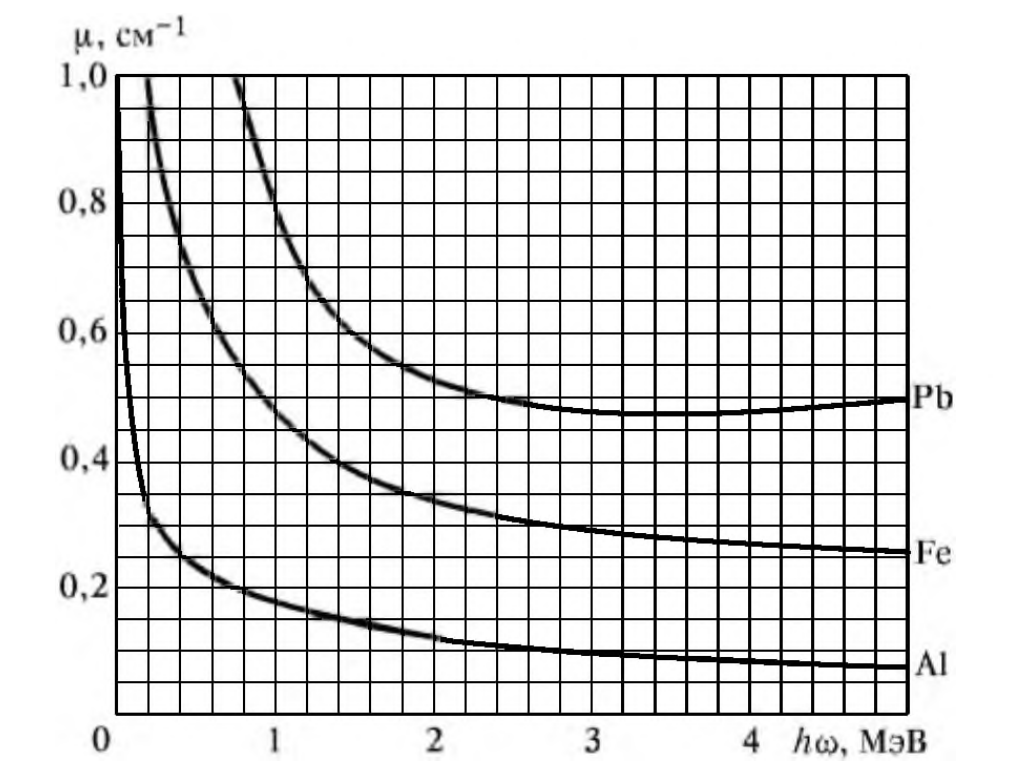
\includegraphics[width=0.5\linewidth]{Screenshot_1}
	\caption{Зависимость полного коэффициента поглощения от энергии $ \gamma $-кванта}
	\label{fig:screenshot1}
\end{figure}

\subsection{Расчётные формулы}

В данной работе коэффициент ослабления $ \mu $ измеряется в хорошей
геометрии, т. е. в условиях, когда исследуется прохождение сквозь вещество узкого параллельного пучка $ \gamma $-лучей.. Из формулы \eqref{eq:exp} имеем
\begin{equation}\label{eq:mu}
	\mu = \frac{1}{l}\ln \frac{N_0}{N}.
\end{equation}

Энергию кванта можно определить по рис. \ref{fig:screenshot1}.

\section{Оборудование и инструментальные погрешности}

Схема экспериментальной установки отображена на рис. \ref{fig:screenshot2}.
Свинцовый коллиматор выделяет узкий почти параллельный пучок $ \gamma $-квантов, проходящий через набор поглотителей П и регистрируемый сцинтилляционным счетчиком. Сигналы от счетчика усиливаются и регистрируются пересчетным прибором ПП. Высоковольтный выпрямитель ВВ обеспечивает питание сцинтилляционного счетчика.
\begin{figure}
	\centering
	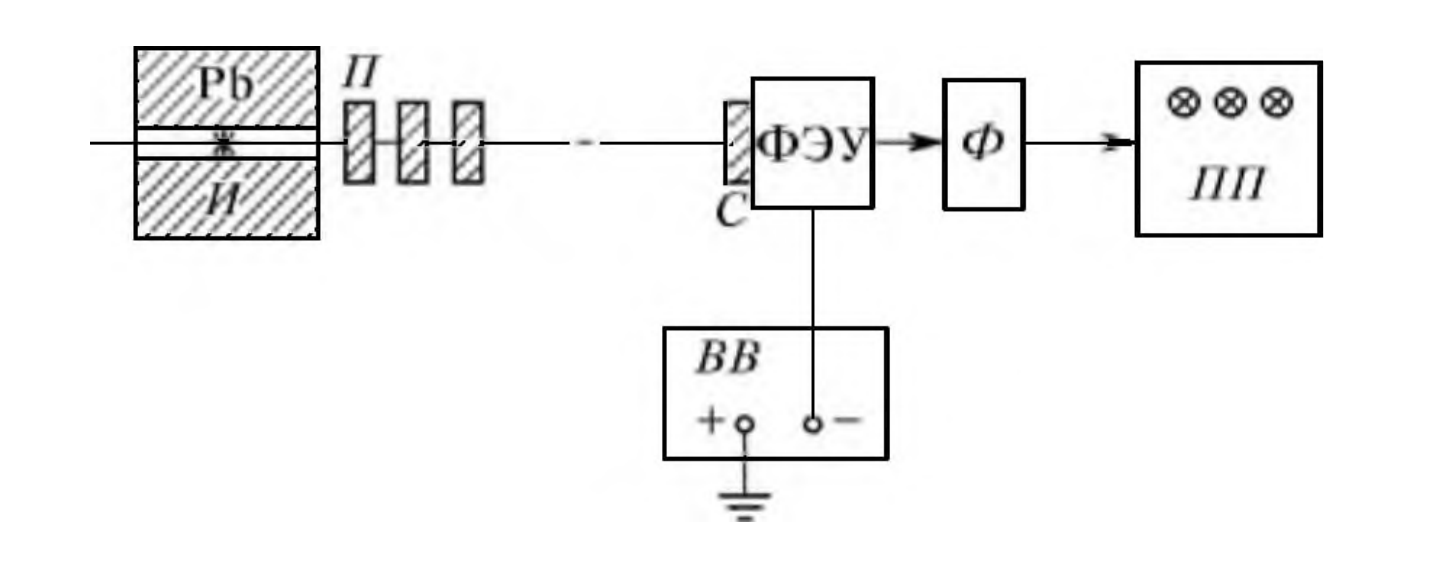
\includegraphics[width=1.0\linewidth]{Screenshot_2}
	\caption{Схема экспериментальной установки}
	\label{fig:screenshot2}
\end{figure}
Поглотители располагаются на расстоянии друг от друга во избежание многократного взаимодействия с ними $ \gamma $-квантов.

В работе используются:
\equip{Источник $ \gamma $-квантов со свинцовым коллиматором}
\equip{Набор поглотителей из различных материалов}
\equip{Сцинтилляционный счётчик}
\equip{Пересчётный прибор}

\section{Результаты измерений и обработка данных}

По результатам проведения опыта получены данные табл. \ref{tab:raw}. Далее необходимо усреднить результаты повторных опытов и найти статистические погрешности отдельного опыта. Учтём наличие фона и соответствующие погрешности. В результате получим данные для построения графиков в табл. \ref{tab:plotData}. Так как требуется график вида $ \ln N_0/N (h) $, погрешность $ \ln N_0/N $ найдём по формуле:
\begin{equation}\label{eq:погрLog}
	\sigma_{log} = \sqrt{\frac{\sigma _N^2}{N^2}+\frac{\sigma _{N_0}^2}{N_0^2}}
\end{equation}

Из графиков на рис. \ref{fig:al}, \ref{fig:fe}, \ref{fig:pb} найдём коэффициенты $ \mu $:
\[
	\mu_{Al} = 0.0203\pm 2*10^{-4} \; мм^{-1},
\]
\[
	\mu_{Fe} = 0.0566\pm 1*10^{-4} \; мм^{-1},
\]	
\[
	\mu_{Pb} = 0.118\pm 0.002 \; мм^{-1}.
\]

\begin{figure}
	\centering
	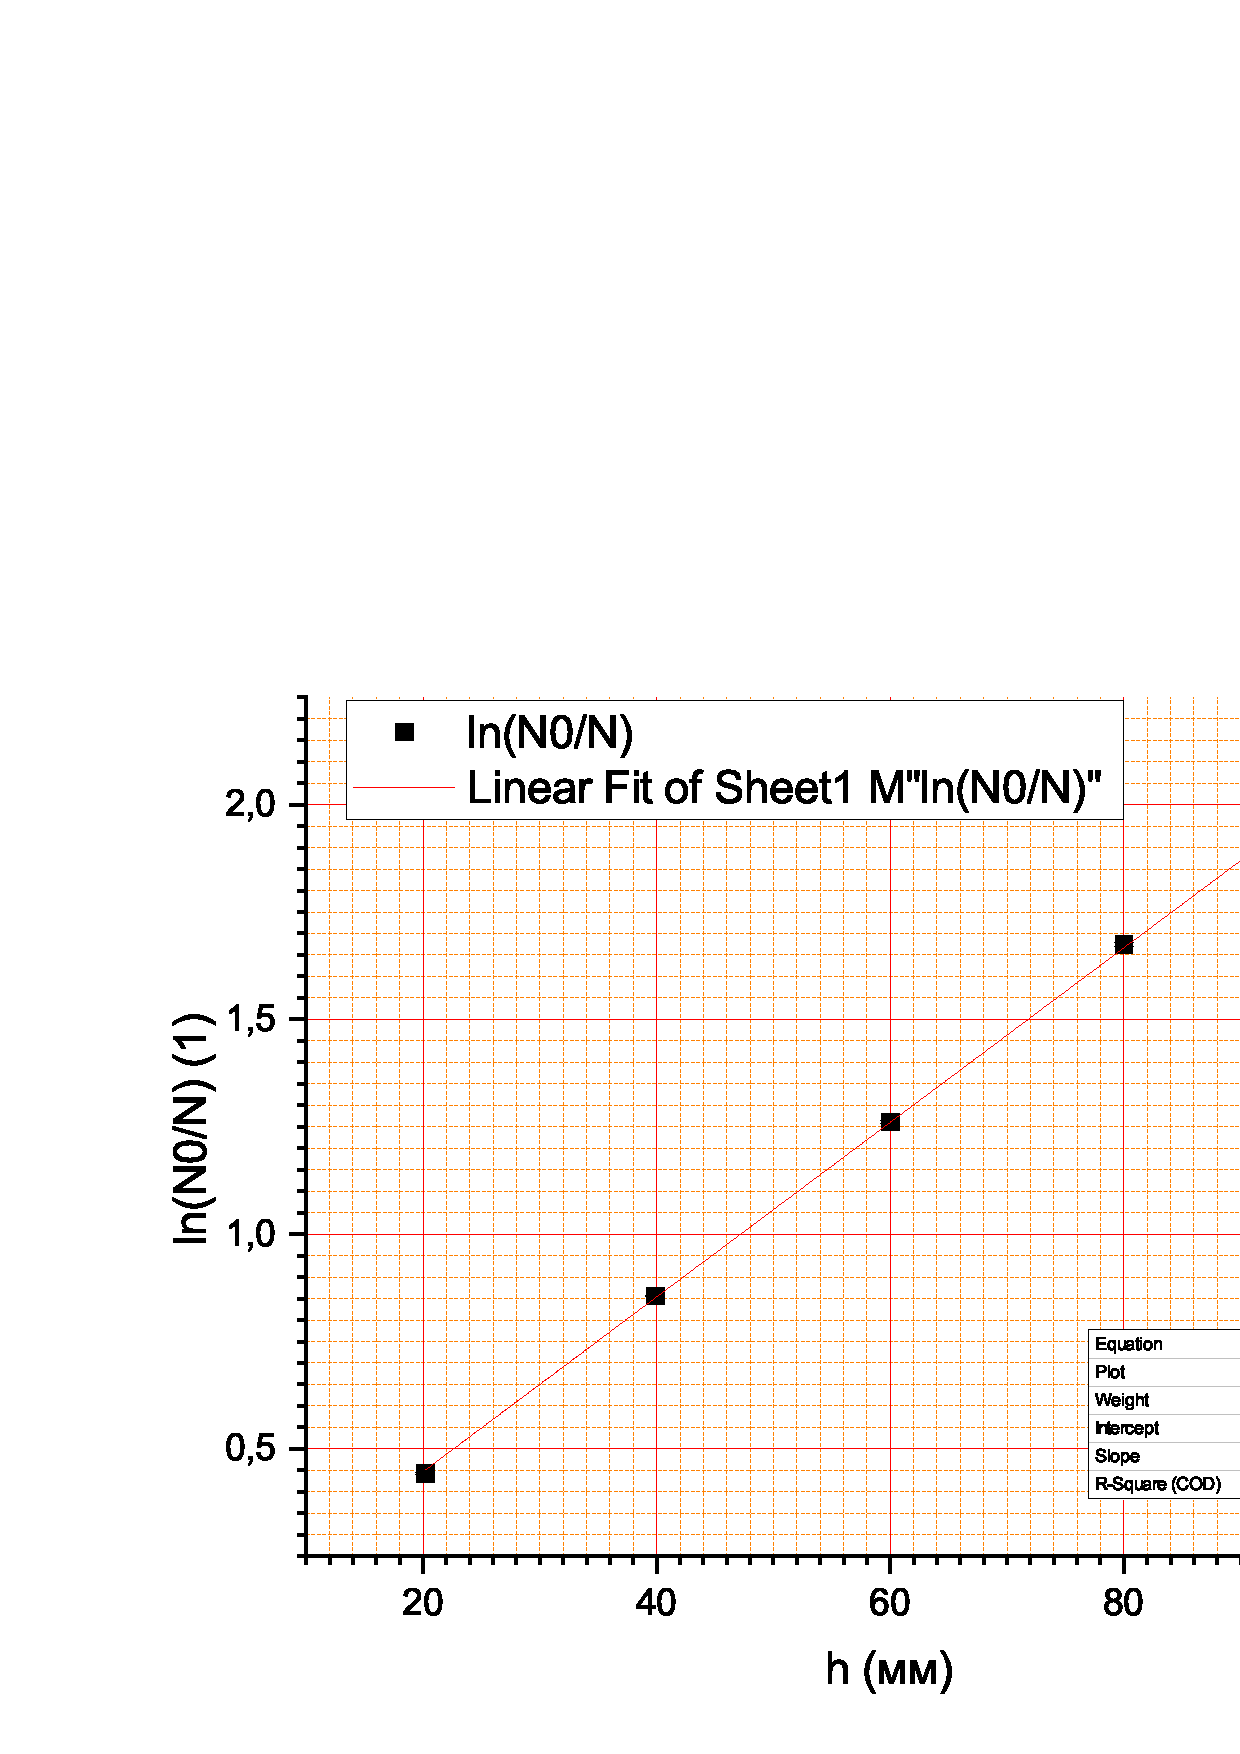
\includegraphics[width=1.0\linewidth]{Al}
	\caption{Зависимость $\ln \frac{N_0}{N} (h)$ для аллюминия}
	\label{fig:al}
\end{figure}

\begin{figure}
	\centering
	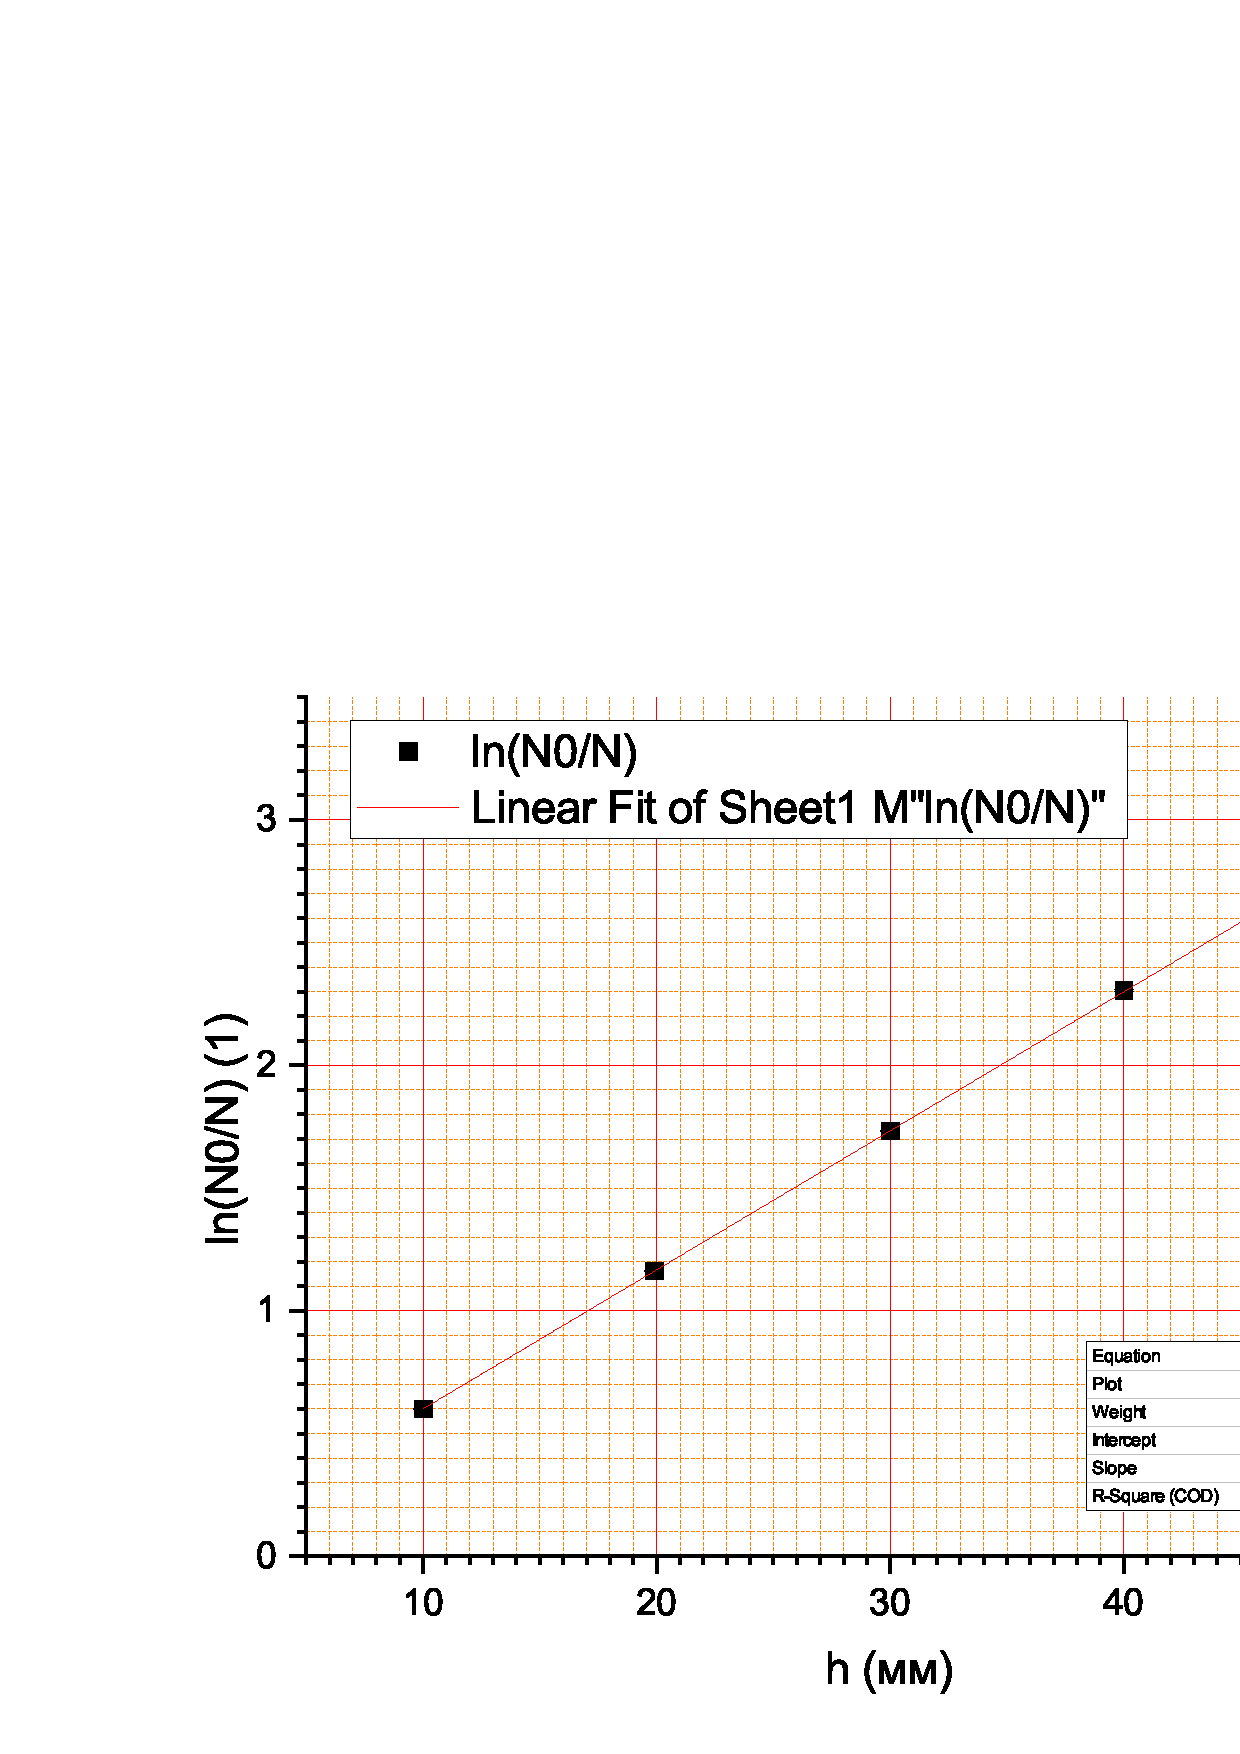
\includegraphics[width=1.0\linewidth]{Fe}
	\caption{Зависимость $\ln \frac{N_0}{N} (h)$ для железа}
	\label{fig:fe}
\end{figure}

\begin{figure}
	\centering
	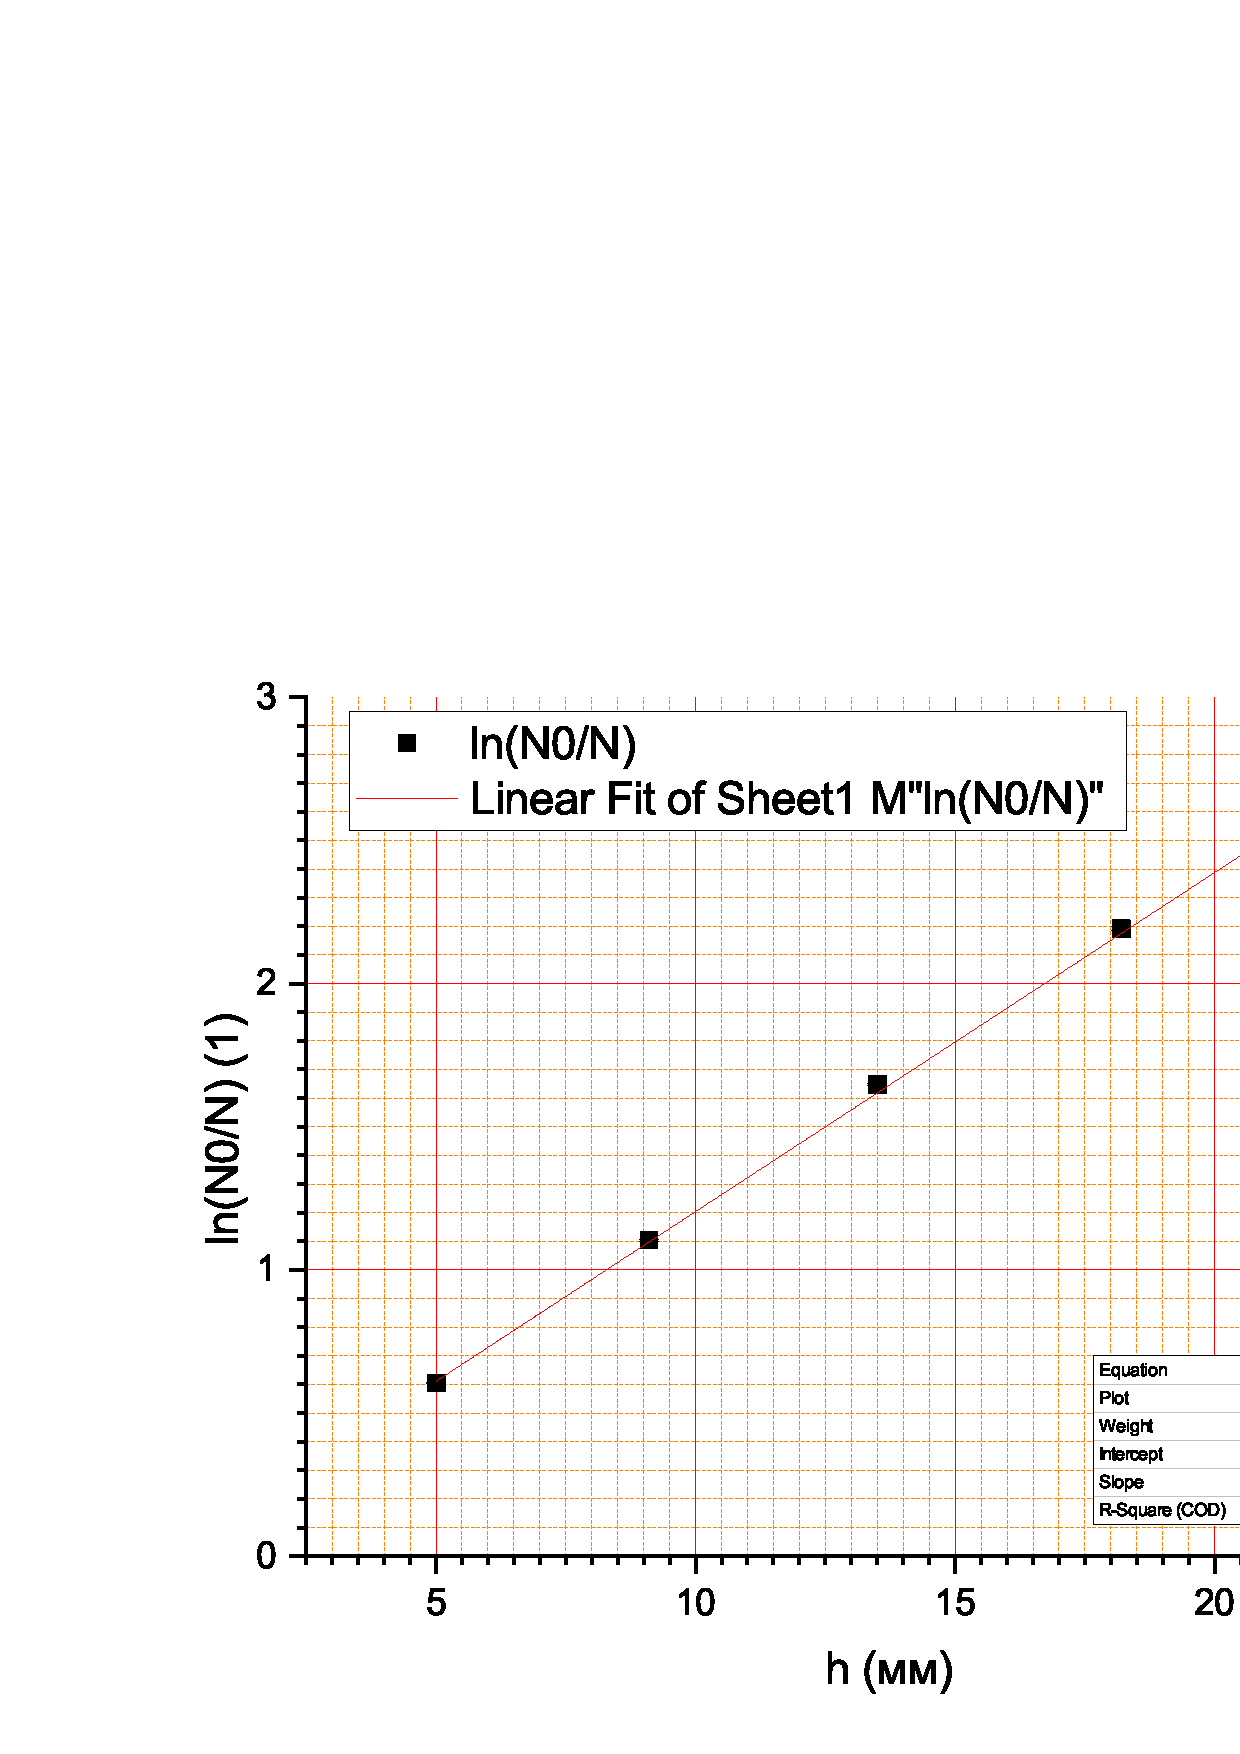
\includegraphics[width=1.0\linewidth]{Pb}
	\caption{Зависимость $\ln \frac{N_0}{N} (h)$ для свинца}
	\label{fig:pb}
\end{figure}

Так как при выполнении лабораторной работы не были замерены диаметры образцов поглотителей, расчёт константы $ \mu' = \mu l /m_1 $ не представляется возможным.

По причине невнимательного прочтения лабника, так же был проведён прямой расчёт по формуле \eqref{eq:mu}. По его результатам,
\[
\mu_{Al} = 0.0211\pm 4*10^{-4} \; мм^{-1},
\]
\[
\mu_{Fe} = 0.0581\pm 7*10^{-4} \; мм^{-1},
\]	
\[
\mu_{Pb} = 0.120\pm 0.008 \; мм^{-1}.
\]
Эти значения приблизительно совпадают с полученными по методу хи-квадрат. Полного совпадения нет, так как расчёт погрешностей по формуле стандартной ошибки среднего даёт более правильный результат при большем количестве опытов.
% Please add the following required packages to your document preamble:
% \usepackage{multirow}
\begin{table}[]
	\centering
	\begin{tabular}{|l|l|l|l|}
		\hline
		Материал & Толщина h & Среднее число $\gamma$-квантов, $N$ & Погрешность среднего, $\sigma_N$ \\ \hline
		\multirow{5}{*}{Аллюминий} & 20.2  & 6,65E+4 & 2E+2 \\ \cline{2-4} 
		& 39.9  & 4,40E+4 & 6E+1 \\ \cline{2-4} 
		& 60.0  & 2,93E+4 & 9E+1 \\ \cline{2-4} 
		& 80.0  & 1,94E+4 & 1E+2 \\ \cline{2-4} 
		& 100.0 & 1,31E+4 & 5E+1 \\ \hline
		\multirow{5}{*}{Железо}    & 10.0  & 5,68E+4 & 1E+2 \\ \cline{2-4} 
		& 19.9  & 3,24E+4 & 8E+1 \\ \cline{2-4} 
		& 30.0  & 1,83E+4 & 5E+1 \\ \cline{2-4} 
		& 40.0  & 1,03E+4 & 4E+1 \\ \cline{2-4} 
		& 50.0  & 5,92E+3 & 4E+1 \\ \hline
		\multirow{5}{*}{Свинец}    & 5.0   & 5,66E+4 & 1E+2 \\ \cline{2-4} 
		& 9.1   & 3,43E+4 & 9E+1 \\ \cline{2-4} 
		& 13.5  & 1,99E+4 & 7E+1 \\ \cline{2-4} 
		& 18.2  & 1,16E+4 & 7E+1 \\ \cline{2-4} 
		& 22.8  & 7,02E+3 & 3E+1 \\ \hline
	\end{tabular}
	\caption{Данные для построения графиков}
	\label{tab:plotData}
\end{table}

Из табл. на стр. 480 \cite{max}, средняя энергия $\gamma$-квантов достигала
\[
	E\approx 0.6 \div 0.8 \; МэВ.
\]
Эти значения подтверждают точность полученных данных, так как $ \mu_{Al} $, $ \mu_{Fe} $ и $ \mu_{Pb} $ соответствуют этой энергии.

\subsection{Оценка погрешностей}

В данной лабораторной по возможности производился учёт всех доступных погрешностей, вне зависимости от их значения. Расчёт наилучшей прямой по методу хи-квадрат с учётом погрешности по обеим осям проведён в \emph{OriginLab}. Расчётные формулы для погрешностей косвенных измерений найдены аналитически в пакете \emph{Wolfram Mathematica} по общей формуле \[\sigma_u^2 = f'^2_{x} \sigma_x^2 + f'^2_x \sigma_x^2 + \ldots. \]

\section{Вывод}

По результатам лабораторной работы получили с хорошей точностью линейные коэффициенты затухания потока $ \gamma $-квантов в различных поглотителях; приблизительно оценили среднюю энергию одиночного $ \gamma $-кванта.

\newpage
\appendix

\section{Необработанные результаты опытов}

\begin{table}[h]
	\centering
	\begin{tabular}{|l|l|l|l|l|l|l|l|l|l|l|}
		\hline
		Число $\gamma$-квантов & 270 & 291 & 287 & 287 & 257 & 239 & 304 & 276 & 285 & 281 \\ \hline
	\end{tabular}
	\caption{Оценка фона}
	\label{tab:rawPhone}
\end{table}

\begin{table}[h]
	\centering
	\begin{tabular}{|l|l|l|l|l|l|}
		\hline
		Число $\gamma$-квантов & 103578 & 103663 & 103895 & 103753 & 103895 \\ \hline
	\end{tabular}
	\caption{Оценка числа падающих $\gamma$-квантов без учёта фона}
	\label{tab:rawN0}
\end{table}

% Please add the following required packages to your document preamble:
% \usepackage{multirow}
\begin{table}[h]
	\centering
	\begin{tabular}{|l|l|l|l|l|l|l|}
		\hline
		Материал                   & Толщина h & \multicolumn{5}{l|}{Число $\gamma$-квантов} \\ \hline
		\multirow{5}{*}{Аллюминий} & 20.2      & 66630   & 66799   & 66902   & 67231  & 66185  \\ \cline{2-7} 
		& 39.9      & 44415   & 44323   & 44348   & 44040  & 44250  \\ \cline{2-7} 
		& 60.0      & 29521   & 29463   & 29566   & 29974  & 29583  \\ \cline{2-7} 
		& 80.0      & 19515   & 19842   & 19389   & 19758  & 19882  \\ \cline{2-7} 
		& 100.0     & 13533   & 13480   & 13465   & 13254  & 13374  \\ \hline
		\multirow{5}{*}{Железо}    & 10.0      & 57257   & 57187   & 56841   & 56771  & 57318  \\ \cline{2-7} 
		& 19.9      & 32497   & 32432   & 32786   & 32821  & 32696  \\ \cline{2-7} 
		& 30.0      & 18527   & 18480   & 18517   & 18696  & 18695  \\ \cline{2-7} 
		& 40.0      & 10654   & 10713   & 10454   & 10637  & 10595  \\ \cline{2-7} 
		& 50.0      & 6122    & 6259    & 6301    & 6123   & 6205   \\ \hline
		\multirow{5}{*}{Свинец}    & 5.0       & 56924   & 56927   & 56663   & 57145  & 56567  \\ \cline{2-7} 
		& 9.1       & 34639   & 34559   & 34534   & 34404  & 34963  \\ \cline{2-7} 
		& 13.5      & 20302   & 20349   & 20240   & 20197  & 19946  \\ \cline{2-7} 
		& 18.2      & 11890   & 11837   & 12046   & 11680  & 11712  \\ \cline{2-7} 
		& 22.8      & 7221    & 7286    & 7395    & 7325   & 7283   \\ \hline
	\end{tabular}
	\caption{Результат эксперимента (сырые данные)}
	\label{tab:raw}
\end{table}


\begin{thebibliography}{3}
	\bibitem{Siv} Сивухин Д. В. \emph{Общий курс физики. Том 5}, 1989
	\bibitem{chp} Фаддеев М. А., Чупрунов Е. В. \emph{Лекции по атомной физике}, 2008
	\bibitem{max} Игошин Ф. Ф., Самарский Ю. А., Ципешок Ю. М. \emph{ЛАБОРАТОРНЫЙ ПРАКТИКУМ ПО ОБЩЕЙ ФИЗИКЕ. Квантовая физика: Учеб, пособие для вузов}; Под ред. Ципенюка Ю.М.
\end{thebibliography}
\end{document}